\section{Auswertung}
\label{sec:Auswertung}

Die Graphen werden sowohl mit Matplotlib \cite{matplotlib} als auch NumPy \cite{numpy} erstellt. Die Fehlerrechnung wird mithilfe von Uncertainties \cite{uncertainties} durchgeführt.

\subsection{Bestimmung der Aktivierungsenergie $W$ bei einer Heizrate von ca. $b=\SI{2}{\kelvin\per\minute}$}

Die erhobenen Messwerte des Polarisationsstroms werden mittels einer Regression der Form
\begin{equation}
I(T)=.e^{a(x-b)} \label{eq:reg1}
\end{equation}
um den zweiten Peak bereinigt. In Abbildung \ref{fig:plot1exp} sind die Rohdaten, die für den Fit verwendeten Werte, sowie der Fit selbst zu sehen.
Für die Parameter ergibt sich:
\begin{align*}
a_1&=\SI{6,02(19)e-2}{\pico\ampere}\\
b_1&=\SI{252,0(16)}{\kelvin}\text{.}
\end{align*}
In Abbildung \ref{fig:bereinigt1} sind die bereinigten Messwerte aufgetragen und in Tabelle \ref{tab:data1} gemeinsam mit den Rohdaten zu sehen.
Für kleine Temperaturen $T$ wird in Abbildung \ref{fig:W1_1} nach Gleichung \eqref{eq:ln1} das Logarithmierte des Polarisationsstrom $i$ gegen das Inverse der Temperatur aufgetragen. Die logarithmischen Werte sind in Tabelle \ref{tab:dataW1_1} eingetragen.
Die lineare Regression
\begin{equation}
\ln\left(\frac{i(T)}{i_.0}\right)=\alpha T^{-1}+\beta \label{eq:reg2}
\end{equation}
liefert die Parameter:
\begin{align*}
\alpha_1&=\SI{-8,63(23)e3}{\kelvin},\\
\beta_1 &= \num{36,3(9)}\text{.}
\end{align*}
Daraus lässt sich die Aktivierungsenergie $W$ berechnen zu:
\[
W_{1,1} = -\alpha_1 k_.B =\SI{1,19(3)e-19}{\joule}=\SI{0.744(19)}{\electronvolt}\text{.}
\]
Die Aktivierungsenergie lässt sich ebenfalls über den gesamten Kurvenverlauf bestimmen. Dazu wird nach Formel \eqref{eq:ln2} eine Ausgleichsrechnung der Form 
\begin{equation}
\ln\left(\frac{\int_T^{T^*} i(T').dT'}{i(T)}\right) = mT^{-1}+n \label{eq:reg3}
\end{equation}
durchgeführt. Dabei ist $T^*=\SI{285,3}{\kelvin}$. Das Integral wird mit der summierten Trapez-Regel approximiert. Es ergeben sich die Parameter:
\begin{align*}
m_1&=\SI{8,90(21)e3}{\kelvin},\\
n_1&=\num{-31,6(8)}\text{.}
\end{align*}
Der Graph ist in Abbildung \ref{fig:W1_2} zu sehen und die zugehörigen Werte in Tabelle \ref{tab:dataW1_2}.
Daraus ergibt sich $W$ zu:
\[
W_{1,2} = m_1 k_.B =\SI{1,23(3)e-19}{\joule}=\SI{0.767(17)}{\electronvolt}\text{.}
\]

\begin{figure}
	\centering
	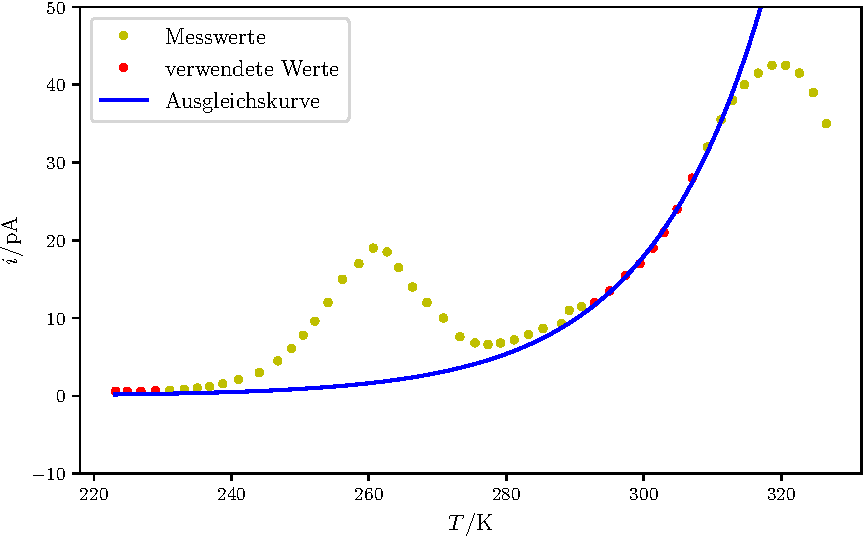
\includegraphics[width=\linewidth-60pt,height=\textheight-60pt,keepaspectratio]{content/images/plot1exp.pdf}
	\caption{Die Messdaten mit der Ausgleichskurve für die ansteigende Flanke des zweiten Peaks.}
	\label{fig:plot1exp}
\end{figure}

\begin{figure}
	\centering
	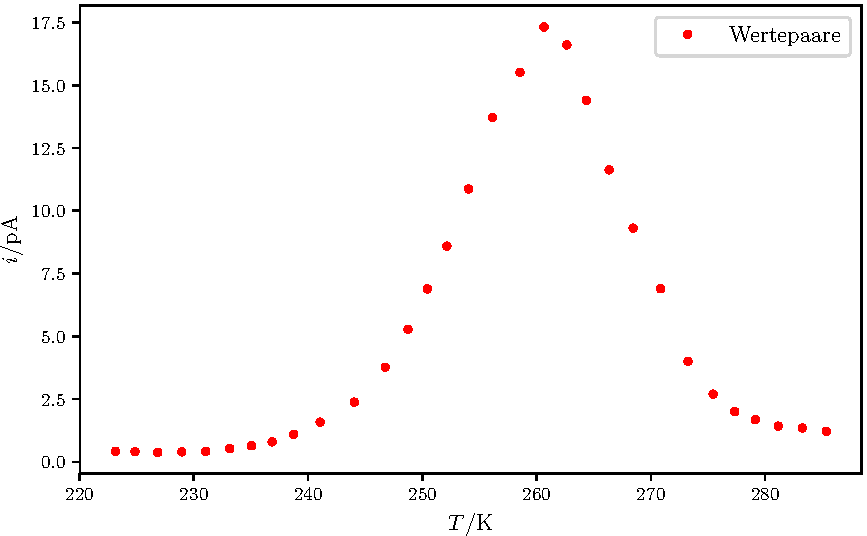
\includegraphics[width=\linewidth-60pt,height=\textheight-60pt,keepaspectratio]{content/images/bereinigt1.pdf}
	\caption{Die bereinigten Messdaten.}
	\label{fig:bereinigt1}
\end{figure}

\begin{table}
\caption{Die bereinigten, als auch die nicht bereinigten Messdaten.}
\begin{minipage}[t]{0.5\textwidth}
	\centering
	\label{tab:tabData1_1}
	\sisetup{table-format=1.2}
	\begin{tabular}{S[table-format=2.0]S[table-format=3.1]S[table-format=2.1]S[table-format=2.1]}
		\toprule
		{$t_\text{1}/(\si{\minute})$} & {$T_\text{1}/(\si{\kelvin})$} & {$i_\text{roh,1}/(\si{\pico\ampere})$} & {$i_\text{ber,1}/(\si{\pico\ampere})$} \\
		\midrule
		 0 & 223.1 & 0.6 & 0.4 \\
		 1 & 224.8 & 0.6 & 0.4 \\
		 2 & 226.8 & 0.6 & 0.4 \\
		 3 & 228.9 & 0.7 & 0.4 \\
		 4 & 231.0 & 0.7 & 0.4 \\
		 5 & 233.1 & 0.8 & 0.5 \\
		 7 & 235.0 & 1.0 & 0.6 \\
		 8 & 236.8 & 1.2 & 0.8 \\
		 9 & 238.7 & 1.6 & 1.1 \\
		10 & 241.0 & 2.1 & 1.6 \\
		11 & 244.0 & 3.0 & 2.4 \\
		12 & 246.7 & 4.5 & 3.8 \\
		13 & 248.7 & 6.1 & 5.3 \\
		14 & 250.4 & 7.8 & 6.9 \\
		15 & 252.1 & 9.6 & 8.6 \\
		16 & 254.0 & 12.0 & 10.9 \\
		17 & 256.1 & 15.0 & 13.7 \\
		18 & 258.5 & 17.0 & 15.5 \\
		19 & 260.6 & 19.0 & 17.3 \\
		20 & 262.6 & 18.5 & 16.6 \\
		21 & 264.3 & 16.5 & 14.4 \\
		22 & 266.3 & 14.0 & 11.6 \\
		23 & 268.4 & 12.0 & 9.3 \\
		24 & 270.8 & 10.0 & 6.9 \\
		25 & 273.2 & 7.6 & 4.0 \\
		26 & 275.4 & 6.8 & 2.7 \\
		\bottomrule
	\end{tabular}

\end{minipage}
\begin{minipage}[t]{0.65\textwidth}
	\centering
	\label{tab:tabData1_2}
	\sisetup{table-format=1.2}
	\begin{tabular}{S[table-format=2.0]S[table-format=3.1]S[table-format=2.1]S[table-format=2.1]}
		\toprule
		{$t_\text{1}/(\si{\minute})$} & {$T_\text{1}/(\si{\kelvin})$} & {$i_\text{roh,1}/(\si{\pico\ampere})$} & {$i_\text{ber,1}/(\si{\pico\ampere})$} \\
		\midrule
		27 & 277.3 & 6.6 & 2.0 \\
		28 & 279.1 & 6.8 & 1.7 \\
		29 & 281.1 & 7.2 & 1.4 \\
		30 & 283.2 & 7.9 & 1.3 \\
		31 & 285.3 & 8.7 & 1.2 \\
		32 & 288.0 & 9.3 & 0.6 \\
		33 & 289.1 & 11.0 & 1.7 \\
		34 & 290.9 & 11.5 & 1.1 \\
		35 & 292.8 & 12.0 & 0.3 \\
		36 & 295.0 & 13.5 & 0.2 \\
		37 & 297.3 & 15.5 & 0.2 \\
		38 & 299.4 & 17.0 & -0.4 \\
		39 & 301.3 & 19.0 & -0.5 \\
		40 & 302.9 & 21.0 & -0.4 \\
		41 & 304.8 & 24.0 & -0.0 \\
		42 & 307.0 & 28.0 & 0.6 \\
		43 & 309.2 & 32.0 & 0.7 \\
		44 & 311.2 & 35.5 & 0.2 \\
		45 & 312.9 & 38.0 & -1.1 \\
		46 & 314.6 & 40.0 & -3.3 \\
		47 & 316.6 & 41.5 & -7.4 \\
		48 & 318.6 & 42.5 & -12.6 \\
		49 & 320.6 & 42.5 & -19.7 \\
		50 & 322.6 & 41.5 & -28.6 \\
		51 & 324.6 & 39.0 & -40.1 \\
		52 & 326.5 & 35.0 & -53.6 \\
		\bottomrule
	\end{tabular}

\end{minipage}
\label{tab:data1}
\end{table}

\begin{figure}
	\centering
	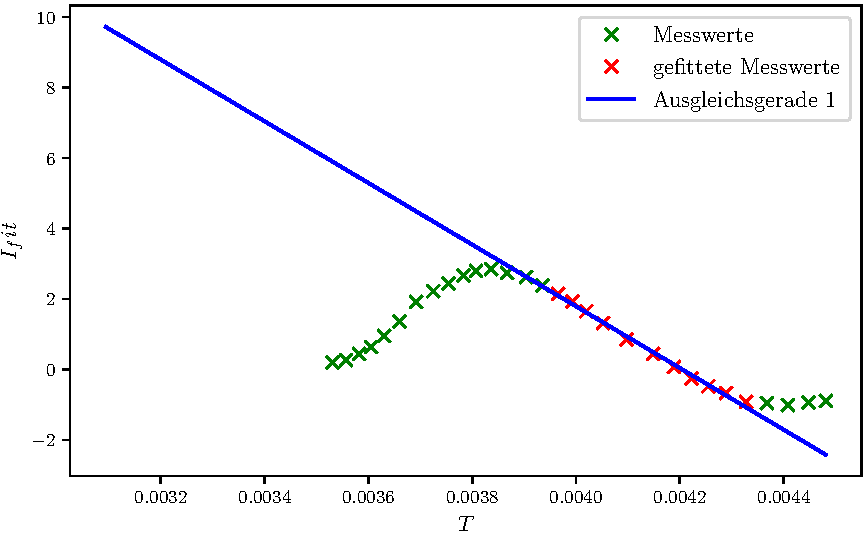
\includegraphics[width=\linewidth-60pt,height=\textheight-60pt,keepaspectratio]{content/images/W1_1.pdf}
	\caption{Die logarithmischen Werte gemäß Formel \eqref{eq:ln1} aufgetragen gegen das Inverse der Temperatur.}
	\label{fig:W1_1}
\end{figure}

\begin{figure}
	\centering
	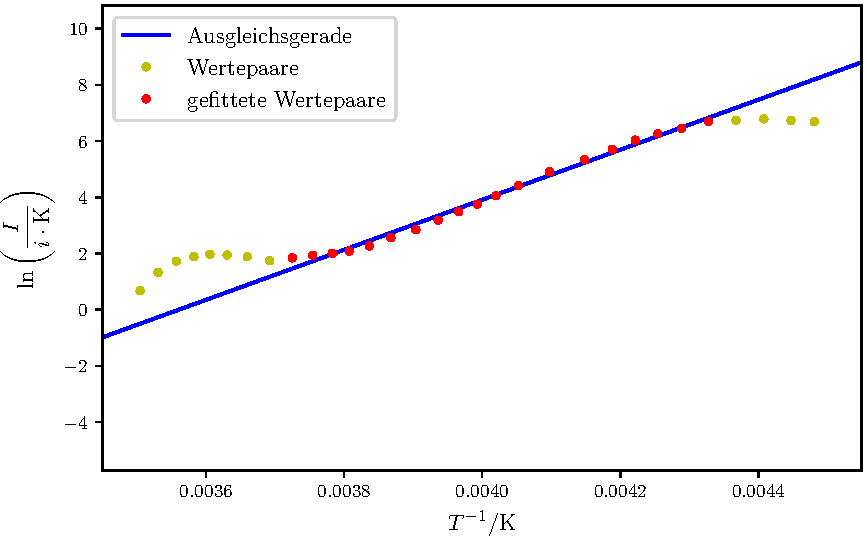
\includegraphics[width=\linewidth-60pt,height=\textheight-60pt,keepaspectratio]{content/images/W1_2.pdf}
	\caption{Die logarithmischen Werte gemäß Formel \eqref{eq:ln2} aufgetragen gegen das Inverse der Temperatur.}
	\label{fig:W1_2}
\end{figure}

\begin{table}
\caption{Die logarithmischen Messdaten gemäß Formel \eqref{eq:ln1} und \eqref{eq:ln2}.}
\begin{minipage}[t]{0.5\textwidth}
%\begin{table}
	\centering
	\label{tab:tabLog11}
	\sisetup{table-format=1.2}
	\begin{tabular}{S[table-format=1.4]S[table-format=1.4]}
		\toprule
		{$T^{-1}_\text{1}/(\si{\kelvin^{-1}})$} & {$\ln{\frac{i_\text{1}}{i_\text{0}}}$} \\
		\midrule
		0.0045 & -0.8587 \\
		0.0044 & -0.9046 \\
		0.0044 & -0.9682 \\
		0.0044 & -0.9161 \\
		0.0043 & -0.8760 \\
		0.0043 & -0.6382 \\
		0.0043 & -0.4474 \\
		0.0042 & -0.2256 \\
		0.0042 & 0.0947 \\
		0.0041 & 0.4590 \\
		0.0041 & 0.8672 \\
		0.0041 & 1.3273 \\
		0.0040 & 1.6635 \\
		0.0040 & 1.9299 \\
		0.0040 & 2.1507 \\
		0.0039 & 2.3859 \\
		0.0039 & 2.6186 \\
		0.0039 & 2.7419 \\
		0.0038 & 2.8517 \\
		0.0038 & 2.8095 \\
		0.0038 & 2.6671 \\
		0.0038 & 2.4535 \\
		0.0037 & 2.2311 \\
		0.0037 & 1.9304 \\
		0.0037 & 1.3887 \\
		0.0036 & 0.9939 \\
		0.0036 & 0.6958 \\
		0.0036 & 0.5188 \\
		0.0036 & 0.3544 \\
		0.0035 & 0.2985 \\
		\bottomrule
	\end{tabular}

	\label{tab:dataW1_1}
%\end{table}
\end{minipage}
\begin{minipage}[t]{0.5\textwidth}
%\begin{table}
	\centering
	\label{tab:tabLog12}
	\sisetup{table-format=1.2}
	\begin{tabular}{S[table-format=1.4]S[table-format=1.4]}
		\toprule
		{$T^{-1}_\text{1}/(\si{\kelvin^{-1}})$} & {$\ln{\frac{I_\text{1}}{i_\text{1}\cdot\si{\kelvin}}}$} \\
		\midrule
		0.0045 & 6.6853 \\
		0.0044 & 6.7290 \\
		0.0044 & 6.7904 \\
		0.0044 & 6.7358 \\
		0.0043 & 6.6932 \\
		0.0043 & 6.4524 \\
		0.0043 & 6.2583 \\
		0.0042 & 6.0326 \\
		0.0042 & 5.7068 \\
		0.0041 & 5.3332 \\
		0.0041 & 4.9067 \\
		0.0041 & 4.4204 \\
		0.0040 & 4.0550 \\
		0.0040 & 3.7540 \\
		0.0040 & 3.4874 \\
		0.0039 & 3.1842 \\
		0.0039 & 2.8479 \\
		0.0039 & 2.5641 \\
		0.0038 & 2.2667 \\
		0.0038 & 2.0820 \\
		0.0038 & 2.0039 \\
		0.0038 & 1.9382 \\
		0.0037 & 1.8429 \\
		0.0037 & 1.7421 \\
		0.0037 & 1.8797 \\
		0.0036 & 1.9446 \\
		0.0036 & 1.9724 \\
		0.0036 & 1.8880 \\
		0.0036 & 1.7241 \\
		0.0035 & 1.3270 \\
		0.0035 & 0.6759 \\
		\bottomrule
	\end{tabular}

	\label{tab:dataW1_2}
%\end{table}
\end{minipage}
\end{table}


\subsection{Bestimmung der Aktivierungsenergie $W$ bei einer Heizrate von ca. $b=\SI{1,4}{\kelvin\per\minute}$}

Die erhobenen Messwerte des Polarisationsstroms werden mittels einer Regression der Form \eqref{eq:reg1} bereinigt. In Abbildung \ref{fig:plot2exp} sind die Rohdaten, die für den Fit verwendeten Werte, sowie der Fit selbst zu sehen.
Für die Parameter ergibt sich:
\begin{align*}
a_2&=\SI{6,24(14)e-2}{\pico\ampere}\\
b_2&=\SI{255,5(11)}{\kelvin}\text{.}
\end{align*}
In Abbildung \ref{fig:bereinigt2} sind die bereinigten Messwerte aufgetragen und in Tabelle \ref{tab:data2} gemeinsam mit den Rohdaten zu sehen.
Für kleine Temperaturen $T$ wird in Abbildung \ref{fig:W2_1} nach Gleichung \eqref{eq:ln1} das Logarithmierte des Polarisationsstrom $i$ gegen das Inverse der Temperatur aufgetragen. Die logarithmischen Werte sind in Tabelle \ref{tab:dataW2_1} eingetragen.
Die lineare Regression der Form \eqref{eq:reg2} liefert die Parameter:
\begin{align*}
\alpha_2&=\SI{-8,29(10)e3}{\kelvin},\\
\beta_2 &= \num{34,9(4)}\text{.}
\end{align*}
Daraus lässt sich die Aktivierungsenergie $W$ berechnen zu:
\[
W_{2,1} = -\alpha_2 k_.B =\SI{1,145(15)e-19}{\joule}=\SI{0.714(8)}{\electronvolt}\text{.}
\]
Die Aktivierungsenergie lässt sich ebenfalls über den gesamten Kurvenverlauf bestimmen. Dazu wird nach Formel \eqref{eq:ln2} eine Ausgleichsrechnung der Form \eqref{eq:reg3} durchgeführt. Dabei ist $T^*=\SI{278,2}{\kelvin}$. Es ergeben sich die Parameter:
\begin{align*}
m_2&=\SI{8,96(11)e3}{\kelvin},\\
n_2&=\SI{-32,4(5)}{}\text{.}
\end{align*}
Der Graph ist in Abbildung \ref{fig:W2_2} zu sehen und die zugehörigen Werte in Tabelle \ref{tab:dataW2_2}.
Daraus ergibt sich $W$ zu:
\[
W_{2,2} = m_2 k_.B =\SI{1,237(14)e-19}{\joule}=\SI{0.772(9)}{\electronvolt}\text{.}
\]

\begin{figure}
	\centering
	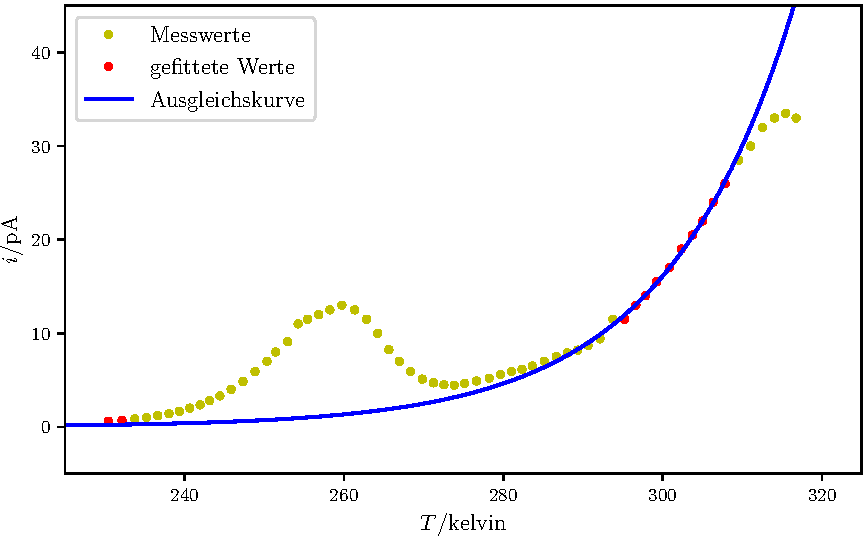
\includegraphics[width=\linewidth-60pt,height=\textheight-60pt,keepaspectratio]{content/images/plot2exp.pdf}
	\caption{Die Messdaten mit der Ausgleichskurve für die ansteigende Flanke des zweiten Peaks.}
	\label{fig:plot2exp}
\end{figure}

\begin{figure}
	\centering
	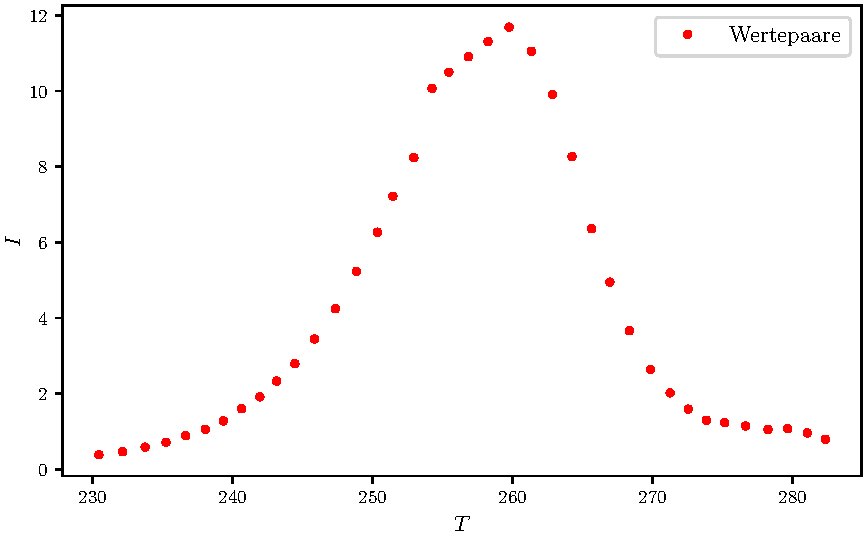
\includegraphics[width=\linewidth-60pt,height=\textheight-60pt,keepaspectratio]{content/images/bereinigt2.pdf}
	\caption{Die bereinigten Messdaten.}
	\label{fig:bereinigt2}
\end{figure}

\begin{table}
\caption{Die bereinigten, als auch die nicht bereinigten Messdaten.}
\begin{minipage}[t]{0.5\textwidth}
	\centering
	\label{tab:tabData2_1}
	\sisetup{table-format=1.2}
	\begin{tabular}{S[table-format=2.0]S[table-format=3.1]S[table-format=2.1]S[table-format=2.1]}
		\toprule
		{$t_\text{2}/(\si{\minute})$} & {$T_\text{2}/(\si{\kelvin})$} & {$i_\text{roh,2}/(\si{\pico\ampere})$} & {$i_\text{ber,2}/(\si{\pico\ampere})$} \\
		\midrule
		 0 & 230.4 & 0.6 & 0.4 \\
		 1 & 232.1 & 0.7 & 0.5 \\
		 2 & 233.7 & 0.8 & 0.6 \\
		 3 & 235.2 & 1.0 & 0.7 \\
		 4 & 236.6 & 1.2 & 0.9 \\
		 5 & 238.0 & 1.4 & 1.1 \\
		 6 & 239.3 & 1.6 & 1.3 \\
		 7 & 240.6 & 2.0 & 1.6 \\
		 8 & 241.9 & 2.4 & 1.9 \\
		 9 & 243.1 & 2.8 & 2.3 \\
		10 & 244.4 & 3.3 & 2.8 \\
		11 & 245.8 & 4.0 & 3.5 \\
		12 & 247.3 & 4.8 & 4.2 \\
		13 & 248.8 & 5.9 & 5.2 \\
		14 & 250.3 & 7.0 & 6.3 \\
		15 & 251.4 & 8.0 & 7.2 \\
		16 & 252.9 & 9.1 & 8.2 \\
		17 & 254.2 & 11.0 & 10.1 \\
		18 & 255.4 & 11.5 & 10.5 \\
		19 & 256.8 & 12.0 & 10.9 \\
		20 & 258.2 & 12.5 & 11.3 \\
		21 & 259.8 & 13.0 & 11.7 \\
		22 & 261.3 & 12.5 & 11.1 \\
		23 & 262.8 & 11.5 & 9.9 \\
		24 & 264.2 & 10.0 & 8.3 \\
		25 & 265.6 & 8.2 & 6.4 \\
		26 & 266.9 & 7.0 & 5.0 \\
		27 & 268.3 & 5.9 & 3.7 \\
		28 & 269.8 & 5.1 & 2.6 \\
		29 & 271.2 & 4.7 & 2.0 \\
		30 & 272.5 & 4.5 & 1.6 \\
		\bottomrule
	\end{tabular}

\end{minipage}
\begin{minipage}[t]{0.65\textwidth}
	\centering
	\label{tab:tabData2_2}
	\sisetup{table-format=1.2}
	\begin{tabular}{S[table-format=2.0]S[table-format=3.1]S[table-format=2.1]S[table-format=2.1]}
		\toprule
		{$t_\text{2}/(\si{\minute})$} & {$T_\text{2}/(\si{\kelvin})$} & {$i_\text{roh,2}/(\si{\pico\ampere})$} & {$i_\text{ber,2}/(\si{\pico\ampere})$} \\
		\midrule
		31 & 273.8 & 1.3 & 1.3 \\
		32 & 275.1 & 1.2 & 1.2 \\
		33 & 276.6 & 1.1 & 1.1 \\
		34 & 278.2 & 1.1 & 1.1 \\
		35 & 279.6 & 1.1 & 1.1 \\
		36 & 281.0 & 1.0 & 1.0 \\
		37 & 282.3 & 0.8 & 0.8 \\
		38 & 283.6 & 0.7 & 0.7 \\
		39 & 285.1 & 0.6 & 0.6 \\
		40 & 286.6 & 0.5 & 0.5 \\
		41 & 288.0 & 0.3 & 0.3 \\
		42 & 289.3 & -0.1 & -0.1 \\
		43 & 290.6 & -0.3 & -0.3 \\
		44 & 292.1 & -0.5 & -0.5 \\
		45 & 293.8 & 0.6 & 0.6 \\
		46 & 295.2 & -0.5 & -0.5 \\
		47 & 296.6 & -0.1 & -0.1 \\
		48 & 297.8 & -0.1 & -0.1 \\
		49 & 299.2 & 0.1 & 0.1 \\
		50 & 300.8 & 0.0 & 0.0 \\
		51 & 302.3 & 0.4 & 0.4 \\
		52 & 303.8 & 0.2 & 0.2 \\
		53 & 305.0 & -0.1 & -0.1 \\
		54 & 306.3 & 0.1 & 0.1 \\
		55 & 307.8 & -0.3 & -0.3 \\
		56 & 309.5 & -0.7 & -0.7 \\
		57 & 311.0 & -2.1 & -2.1 \\
		58 & 312.5 & -3.2 & -3.2 \\
		59 & 314.0 & -5.7 & -5.7 \\
		60 & 315.4 & -8.7 & -8.7 \\
		61 & 316.8 & -12.7 & -12.7 \\
		\bottomrule
	\end{tabular}

\end{minipage}
\label{tab:data2}
\end{table}

\begin{figure}
	\centering
	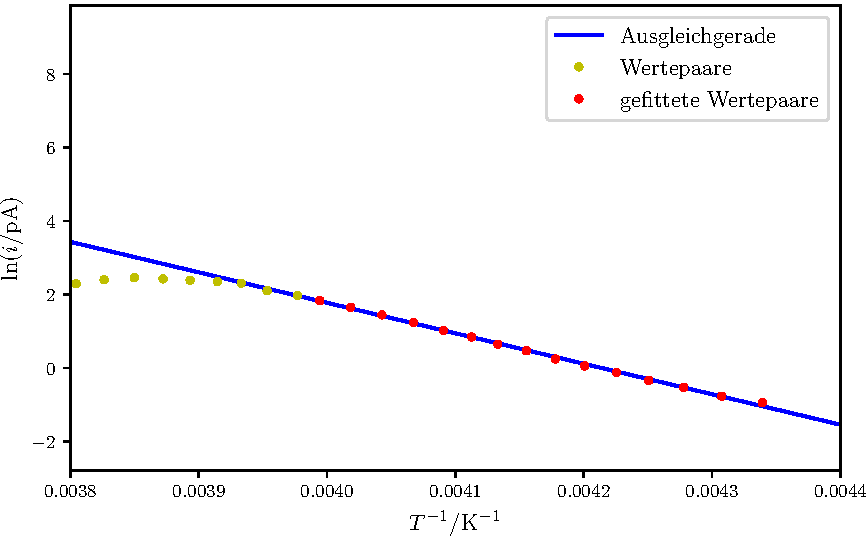
\includegraphics[width=\linewidth-60pt,height=\textheight-60pt,keepaspectratio]{content/images/W2_1.pdf}
	\caption{Die logarithmischen Werte gemäß Formel \eqref{eq:ln1} aufgetragen gegen das Inverse der Temperatur.}
	\label{fig:W2_1}
\end{figure}

\begin{figure}
	\centering
	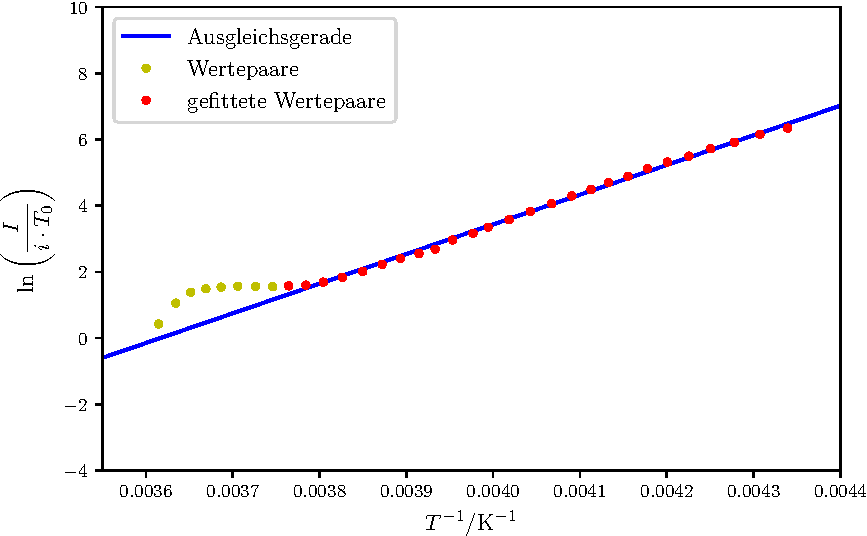
\includegraphics[width=\linewidth-60pt,height=\textheight-60pt,keepaspectratio]{content/images/W2_2.pdf}
	\caption{Die logarithmischen Werte gemäß Formel \eqref{eq:ln2} aufgetragen gegen das Inverse der Temperatur.}
	\label{fig:W2_2}
\end{figure}

\begin{table}
\caption{Die logarithmischen Messdaten gemäß Formel \eqref{eq:ln1} und \eqref{eq:ln2}.}
\begin{minipage}[t]{0.5\textwidth}
%\begin{table}
	\centering
	\label{tab:tabLog21}
	\sisetup{table-format=1.2}
	\begin{tabular}{S[table-format=1.4]S[table-format=1.4]}
		\toprule
		{$T^{-1}_\text{2}/(\si{\kelvin^{-1}})$} & {$\ln{\frac{i_\text{2}}{i_\text{0}}}$} \\
		\midrule
		0.0043 & -0.9420 \\
		0.0043 & -0.7628 \\
		0.0043 & -0.5245 \\
		0.0043 & -0.3334 \\
		0.0042 & -0.1158 \\
		0.0042 & 0.0605 \\
		0.0042 & 0.2499 \\
		0.0042 & 0.4719 \\
		0.0041 & 0.6520 \\
		0.0041 & 0.8484 \\
		0.0041 & 1.0285 \\
		0.0041 & 1.2386 \\
		0.0040 & 1.4462 \\
		0.0040 & 1.6559 \\
		0.0040 & 1.8362 \\
		0.0040 & 1.9770 \\
		0.0040 & 2.1096 \\
		0.0039 & 2.3098 \\
		0.0039 & 2.3514 \\
		0.0039 & 2.3896 \\
		0.0039 & 2.4257 \\
		0.0038 & 2.4590 \\
		0.0038 & 2.4030 \\
		0.0038 & 2.2940 \\
		0.0038 & 2.1126 \\
		0.0038 & 1.8503 \\
		0.0037 & 1.5998 \\
		0.0037 & 1.2989 \\
		0.0037 & 0.9731 \\
		0.0037 & 0.7042 \\
		\bottomrule
	\end{tabular}

	\label{tab:dataW2_1}
%\end{table}
\end{minipage}
\begin{minipage}[t]{0.5\textwidth}
%\begin{table}
	\centering
	\label{tab:tabLog22}
	\sisetup{table-format=1.2}
	\begin{tabular}{S[table-format=1.4]S[table-format=1.4]}
		\toprule
		{$T^{-1}_\text{2}/(\si{\kelvin^{-1}})$} & {$\ln{\frac{I_\text{2}}{i_\text{2}\cdot\si{\kelvin}}}$} \\
		\midrule
		0.0043 & 6.3415 \\
		0.0043 & 6.1591 \\
		0.0043 & 5.9169 \\
		0.0043 & 5.7213 \\
		0.0042 & 5.4986 \\
		0.0042 & 5.3159 \\
		0.0042 & 5.1195 \\
		0.0042 & 4.8888 \\
		0.0041 & 4.6978 \\
		0.0041 & 4.4892 \\
		0.0041 & 4.2930 \\
		0.0041 & 4.0612 \\
		0.0040 & 3.8244 \\
		0.0040 & 3.5774 \\
		0.0040 & 3.3499 \\
		0.0040 & 3.1668 \\
		0.0040 & 2.9641 \\
		0.0039 & 2.6864 \\
		0.0039 & 2.5576 \\
		0.0039 & 2.4022 \\
		0.0039 & 2.2280 \\
		0.0038 & 2.0152 \\
		0.0038 & 1.8387 \\
		0.0038 & 1.6912 \\
		0.0038 & 1.6026 \\
		0.0038 & 1.5780 \\
		0.0037 & 1.5559 \\
		0.0037 & 1.5597 \\
		0.0037 & 1.5688 \\
		0.0037 & 1.5403 \\
		\bottomrule
	\end{tabular}

	\label{tab:dataW2_2}
%\end{table}
\end{minipage}
\end{table}

\subsection{Bestimmung der charakteristischen Relaxatioszeit $\tau_0$}

Zur Bestimmung der charakteristischen Relaxationszeit $\tau_0$ werden die zuvor ermittelten Werte von $W$ mit der Formel für den Mittelwert
\[
\mu_W = \frac{1}{N}\sum_{i=1}^{N}W_i
\]
und dessen Standartabweichung
\[
\sigma_W = \sqrt{\frac{1}{N(N-1)}\sum_{i=1}^{N}(W_i-\mu_W)^2}
\]
gemittelt zu:
\[
W = \mu_W \pm \sigma_W = \SI{1,200(21)e-19}{\joule} = \SI{0.749(13)}{\electronvolt}\text{.}
\]
Zudem werden die Heizraten mithilfe der Werte aus den Tabellen \ref{tab:data1} und \ref{tab:data2} gemittelt zu:
\begin{align*}
b_1 &= \SI{1,95(7)}{\kelvin\per\minute},\\
b_2 &= \SI{1,39(3)}{\kelvin\per\minute}\text{.} 
\end{align*}
Damit ergeben sich mit Formel \eqref{eq:tau0} und mit $T_.{max,1}=\SI{260,65}{\kelvin}$ und $T_.{max,2}=\SI{259,75}{\kelvin}$, welche den Messdaten entnommen werden, für die $\tau_0$:
\begin{align*}
\tau_{0,1} &= \SI{0,8(5)e-12}{\second},\\
\tau_{0,2} &= \SI{1,0(6)e-12}{\second}\text{.}
\end{align*}
Der Fehler $\sigma_.{\tau}$ berechnet sich dabei nach der Gaußschen Fehlerfortpflanzung über
\[
\sigma_.{\tau}=\sqrt{\frac{(k_.BT^2_.{max})^2}{W^2b^4}.e^{-\frac{2 W}{k_.BT_.{max}}}\cdot\sigma^2_.b+\frac{T^2_.{max}(k_.BT_.{max}+W)^2}{W^4b^2}.e^{-\frac{2 W}{k_.BT_.{max}}}\cdot\sigma^2_.W}\text{.}
\]
